\section{Spending Analysis}

\subsection{Cost Drivers}
Figure~\ref{fig:cost_drivers} summarises the main cost components per request.
\begin{itemize}
    \item \textbf{OpenAI}: GPT-4o-mini (or configured model) is charged per token (input and output). Each user question and the system/party context consume input tokens; the JSON array of messages is output. Whisper is charged per minute of audio for \texttt{/sts} \textcite{openai_pricing}.
    \item \textbf{ElevenLabs}: Usage is typically metered by characters or by time of generated audio, depending on plan \textcite{elevenlabs_pricing}. Every non-default reply triggers one TTS call per message (up to three per request).
    \item \textbf{Local compute}: ffmpeg and Rhubarb run locally; cost is negligible compared to APIs but adds to hosting if scaled.
\end{itemize}

\begin{figure}[H]
\centering
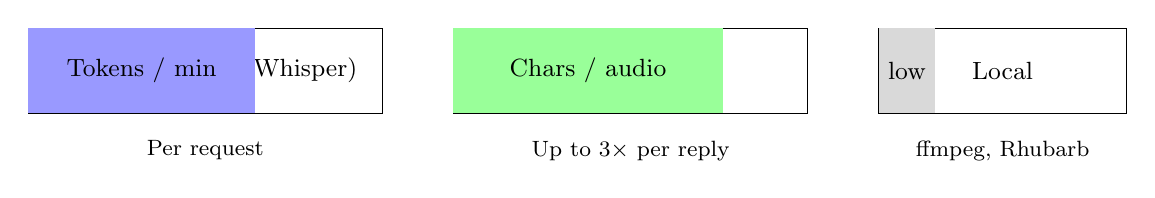
\begin{tikzpicture}[scale=0.9, every node/.style={font=\small}]
    \draw (0,0) rectangle (5,1.2);
    \node at (2.5,0.6) {OpenAI (LLM + Whisper)};
    \fill [blue!40] (0,0) rectangle (3.2,1.2);
    \node at (1.6,0.6) {Tokens / min};
    \draw (6,0) rectangle (11,1.2);
    \node at (8.5,0.6) {ElevenLabs TTS};
    \fill [green!40] (6,0) rectangle (9.8,1.2);
    \node at (7.9,0.6) {Chars / audio};
    \draw (12,0) rectangle (15.5,1.2);
    \node at (13.75,0.6) {Local};
    \fill [gray!30] (12,0) rectangle (12.8,1.2);
    \node at (12.4,0.6) {low};
    \node [below, font=\footnotesize] at (2.5,-0.25) {Per request};
    \node [below, font=\footnotesize] at (8.5,-0.25) {Up to 3$\times$ per reply};
    \node [below, font=\footnotesize] at (13.75,-0.25) {ffmpeg, Rhubarb};
\end{tikzpicture}
\caption[Cost drivers]{Main cost drivers: OpenAI (input/output tokens and Whisper minutes), ElevenLabs (per character or audio length, multiplied by message count), and negligible local compute.}
\label{fig:cost_drivers}
\end{figure}

\subsection{Weaknesses in Spending}
\begin{enumerate}
    \item \textbf{No caching}: Identical or repeated questions (or default-responses logic) still go through the full pipeline when they are not caught by the default-message check. No caching of LLM responses or TTS output for the same text.
    \item \textbf{No tiering}: Every request uses the same model and TTS settings; there is no option to use a cheaper/faster model for simple queries or fallback when rate-limited.
    \item \textbf{Redundant TTS}: If the same phrase appears in different conversations (e.g.\ error or fallback messages), it is re-synthesised every time. The default “API keys missing” and “I didn’t catch that” paths use pre-generated files only when those exact flows are hit; any other path always calls ElevenLabs.
    \item \textbf{Whisper on every STS}: Every speech input is sent to Whisper; there is no short-audio or low-confidence path to avoid transcription cost.
    \item \textbf{Multiple messages}: Cap of 3 messages per turn multiplies TTS and phoneme cost by up to 3 compared to a single-sentence reply.
\end{enumerate}
